% Standalone preview of 5 alternative layouts for Figure 2.
% Compile: pdflatex preview-overview-alts.tex
\documentclass{article}
\usepackage[a4paper,landscape,margin=1.5cm]{geometry}
\usepackage{tikz}
\usepackage{xcolor}
\usepackage{caption}
\usetikzlibrary{arrows.meta, calc}

% Ontology name
\newcommand{\OurOntology}{MLIPO}

% Ontology notations
\newcommand{\concept}[1]{\mathsf{#1}}
\newcommand{\role}[1]{\mathsf{#1}}

% Ontology vocabulary
\newcommand{\MLIP}{\concept{MLIP}}
\newcommand{\MTP}{\concept{MTP}}
\newcommand{\Simulation}{\concept{Simulation}}
\newcommand{\SimulationCell}{\concept{SimulationCell}}
\newcommand{\hasState}{\role{hasState}}
\newcommand{\initialState}{\role{initialState}}
\newcommand{\finalState}{\role{finalState}}
\newcommand{\nextState}{\role{nextState}}
\newcommand{\pointInTime}{\role{pointInTime}}
\newcommand{\energyModel}{\role{energyModel}}
\newcommand{\forcesModel}{\role{forcesModel}}


\definecolor{algofill}{HTML}{A6CEE3}
\definecolor{trainfill}{HTML}{B2DF8A}
\definecolor{benchfill}{HTML}{FDBF6F}

\setlength{\parindent}{0pt}

\begin{document}

\section*{Figure 2 — alternative layouts (5 variants)}

Each variant adds the four leaf classes (DatasetProvenance,
CoveredProperty, MetricType, MetricProperty) and the
\texttt{trainedWith} shortcut (drawn dotted) currently missing from
Fig. 2. The five variants differ in where the new classes are placed
and how the \texttt{trainedWith} arc is routed.

\bigskip

\textbf{Alt 1.} New leaf row: all four new classes on a single bottom
row at $y=-0.8$. \texttt{trainedWith}: long arc on the LEFT of the
central column.\\[0.3em]
\centering
\resizebox{\textwidth}{!}{\input{artifacts/figures/mlips-overview-alt1.tex}}

\newpage
\raggedright
\textbf{Alt 2.} Right-column extension: dataset leaves below
TrainingDataset; metric leaves stacked vertically to the RIGHT of
AccuracyMetric (new column at $x=17$). \texttt{trainedWith}: arc on the
RIGHT of the central column.\\[0.3em]
\centering
\resizebox{\textwidth}{!}{\input{artifacts/figures/mlips-overview-alt2.tex}}

\newpage
\raggedright
\textbf{Alt 3.} Stacks below each parent: DatasetProvenance directly
below TrainingDataset, then CoveredProperty below it; same for
MetricType + MetricProperty below AccuracyMetric. Two extra rows are
added (at $y=-0.8$ and $y=-2.0$). \texttt{trainedWith}: arc on the
LEFT.\\[0.3em]
\centering
\resizebox{\textwidth}{!}{\input{artifacts/figures/mlips-overview-alt3.tex}}

\newpage
\raggedright
\textbf{Alt 4.} Pairs side-by-side below each parent: dataset leaves
side-by-side below TrainingDataset; metric leaves side-by-side below
AccuracyMetric. Single new row at $y=-0.8$. \texttt{trainedWith}: short
tight arc on the RIGHT of the central column.\\[0.3em]
\centering
\resizebox{\textwidth}{!}{\input{artifacts/figures/mlips-overview-alt4.tex}}

\newpage
\raggedright
\textbf{Alt 5.} Hybrid: dataset leaves below TrainingDataset; metric
leaves spread horizontally below the right side (using free space
under DFTSettings). \texttt{trainedWith}: arc on the RIGHT.\\[0.3em]
\centering
\resizebox{\textwidth}{!}{% ALT 5: Hybrid — dataset leaves below, metric leaves stacked at top right.
% DatasetProvenance + CoveredProperty: side-by-side below TrainingDataset.
% MetricType + MetricProperty: vertically stacked ABOVE AccuracyMetric
%   (filling unused space above HyperparameterSetting on the right).
% trainedWith shortcut: dotted arc on the LEFT of the central column,
%   passing through the corridor between the central and left columns.
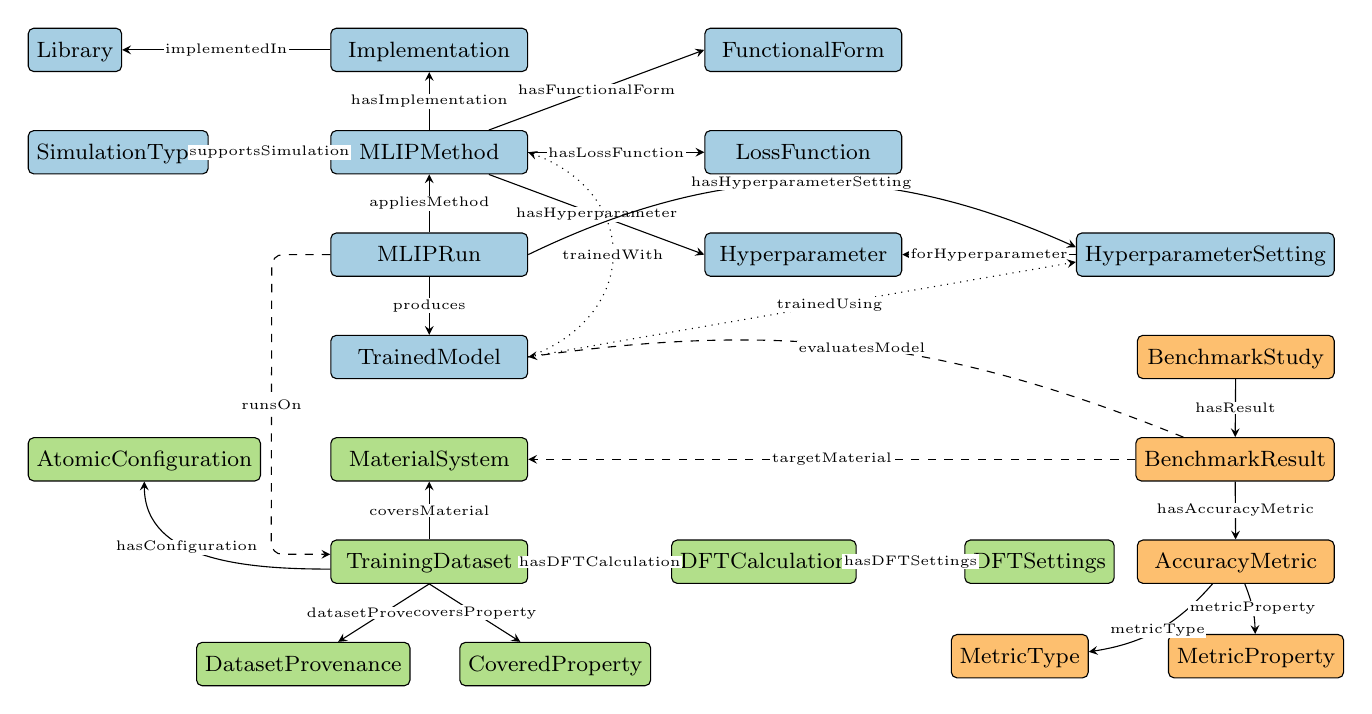
\begin{tikzpicture}[
    x=1cm, y=1cm,
    every node/.style={font=\footnotesize},
    methodnode/.style={draw, rounded corners=2pt, fill=algofill,
        minimum height=0.55cm, inner sep=3pt, align=center,
        font=\footnotesize, text height=1.6ex, text depth=0.4ex},
    trainnode/.style={draw, rounded corners=2pt, fill=trainfill,
        minimum height=0.55cm, inner sep=3pt, align=center,
        font=\footnotesize, text height=1.6ex, text depth=0.4ex},
    benchnode/.style={draw, rounded corners=2pt, fill=benchfill,
        minimum height=0.55cm, inner sep=3pt, align=center,
        font=\footnotesize, text height=1.6ex, text depth=0.4ex},
    centerwidth/.style={minimum width=2.5cm},
    edge/.style={->, >=stealth, thin},
    crossedge/.style={->, >=stealth, thin, dashed},
    shortcut/.style={->, >=stealth, thin, dotted},
    edgelabel/.style={font=\tiny, fill=white, inner sep=0.5pt},
]
  \node[methodnode, centerwidth] (Implementation)  at (5, 7.0) {Implementation};
  \node[methodnode, centerwidth] (MLIPMethod)      at (5, 5.7) {MLIPMethod};
  \node[methodnode, centerwidth] (MLIPRun)         at (5, 4.4) {MLIPRun};
  \node[methodnode, centerwidth] (TrainedModel)    at (5, 3.1) {TrainedModel};
  \node[trainnode,  centerwidth] (MaterialSystem)  at (5, 1.8) {MaterialSystem};
  \node[trainnode,  centerwidth] (TrainingDataset) at (5, 0.5) {TrainingDataset};
  \node[methodnode, anchor=west] (Library)              at (-0.1, 7.0) {Library};
  \node[methodnode, anchor=west] (SimulationType)       at (-0.1, 5.7) {SimulationType};
  \node[trainnode,  anchor=west] (AtomicConfiguration)  at (-0.1, 1.8) {AtomicConfiguration};
  \node[methodnode, anchor=east] (HyperparameterSetting) at (16.5, 4.4) {HyperparameterSetting};
  \node[benchnode,  anchor=east, minimum width=2.5cm] (BenchmarkStudy)  at (16.5, 3.1) {BenchmarkStudy};
  \node[benchnode,  anchor=east, minimum width=2.5cm] (BenchmarkResult) at (16.5, 1.8) {BenchmarkResult};
  \node[benchnode,  anchor=east, minimum width=2.5cm] (AccuracyMetric)  at (16.5, 0.5) {AccuracyMetric};
  \node[methodnode, minimum width=2.5cm] (FunctionalForm) at (9.75, 7.0) {FunctionalForm};
  \node[methodnode, minimum width=2.5cm] (LossFunction)   at (9.75, 5.7) {LossFunction};
  \node[methodnode, minimum width=2.5cm] (Hyperparameter) at (9.75, 4.4) {Hyperparameter};
  \node[trainnode] (DFTCalculation)  at (9.25,  0.5) {DFTCalculation};
  \node[trainnode] (DFTSettings)     at (12.75, 0.5) {DFTSettings};

  % NEW LEAF NODES
  % Dataset leaves below TrainingDataset (side-by-side)
  \node[trainnode] (DatasetProvenance) at (3.4, -0.8) {DatasetProvenance};
  \node[trainnode] (CoveredProperty)   at (6.6, -0.8) {CoveredProperty};
  % Metric leaves: stacked vertically below AccuracyMetric, but with
  % MetricType reaching up between rows (uses available horizontal
  % space at x=12.5 below DFTSettings)
  \node[benchnode] (MetricType)     at (12.5, -0.7) {MetricType};
  \node[benchnode] (MetricProperty) at (15.5, -0.7) {MetricProperty};

  \draw[edge] (MLIPMethod) -- node[edgelabel] {hasFunctionalForm} (FunctionalForm.west);
  \draw[edge] (MLIPMethod) -- node[edgelabel] {hasLossFunction} (LossFunction.west);
  \draw[edge] (MLIPMethod) -- node[edgelabel] {hasHyperparameter} (Hyperparameter.west);
  \draw[edge] (MLIPMethod) -- node[edgelabel] {hasImplementation} (Implementation);
  \draw[edge] (MLIPMethod) -- node[edgelabel] {supportsSimulation} (SimulationType);
  \draw[edge] (Implementation) -- node[edgelabel] {implementedIn} (Library);
  \draw[edge] (HyperparameterSetting) -- node[edgelabel] {forHyperparameter} (Hyperparameter.east);
  \draw[edge] (MLIPRun) -- node[edgelabel] {appliesMethod} (MLIPMethod);
  \draw[edge] (MLIPRun) -- node[edgelabel] {produces} (TrainedModel.north);
  \draw[edge] (TrainingDataset) -- node[edgelabel] {hasDFTCalculation} (DFTCalculation);
  \draw[edge] (TrainingDataset) -- node[edgelabel] {coversMaterial} (MaterialSystem);
  \draw[edge] ($(TrainingDataset.north west)!2/3!(TrainingDataset.south west)$)
    to[out=180, in=270] node[edgelabel, pos=0.6] {hasConfiguration} (AtomicConfiguration.south);
  \draw[edge] (DFTCalculation) -- node[edgelabel] {hasDFTSettings} (DFTSettings);
  \draw[edge] (BenchmarkStudy) -- node[edgelabel] {hasResult} (BenchmarkResult);
  \draw[edge] (BenchmarkResult) -- node[edgelabel] {hasAccuracyMetric} (AccuracyMetric);

  % NEW EDGES
  \draw[edge] (TrainingDataset.south) -- node[edgelabel] {datasetProvenance} (DatasetProvenance);
  \draw[edge] (TrainingDataset.south) -- node[edgelabel] {coversProperty} (CoveredProperty);
  \draw[edge] (AccuracyMetric) to[bend left=20] node[edgelabel, pos=0.5] {metricType} (MetricType);
  \draw[edge] (AccuracyMetric) to[bend left=10] node[edgelabel, pos=0.5] {metricProperty} (MetricProperty);

  \coordinate (runsOnEnd) at ($(TrainingDataset.north west)!1/3!(TrainingDataset.south west)$);
  \coordinate (runsOnTurn) at ($(runsOnEnd) + (-0.75, 0)$);
  \draw[crossedge, rounded corners=4pt] (MLIPRun.west) -- (3, 4.4) --
    node[edgelabel] {runsOn} (runsOnTurn) -- (runsOnEnd);
  \draw[crossedge, bend right=15] (BenchmarkResult) to
    node[edgelabel, pos=0.5] {evaluatesModel} (TrainedModel.east);
  \draw[crossedge] (BenchmarkResult) -- node[edgelabel] {targetMaterial} (MaterialSystem);

  % HyperparameterSetting incoming: solid from MLIPRun (underlying), dotted
  % shortcut from TrainedModel. Endpoints split at 1/3 vs 2/3 down its west
  % side to avoid overlap.
  \draw[edge, bend left=25] (MLIPRun.east) to
    node[edgelabel, pos=0.5] {hasHyperparameterSetting}
    ($(HyperparameterSetting.north west)!1/3!(HyperparameterSetting.south west)$);
  \draw[shortcut] (TrainedModel.east) to
    node[edgelabel, pos=0.55] {trainedUsing}
    ($(HyperparameterSetting.north west)!2/3!(HyperparameterSetting.south west)$);

  % trainedWith shortcut: dotted arc on the right, threading between
  % the central column and the right-of-method column.
  \draw[shortcut, bend right=70, looseness=1.5]
    (TrainedModel.east) to node[edgelabel, pos=0.5] {trainedWith} (MLIPMethod.east);
\end{tikzpicture}
}

\end{document}
